\begin{figure}[!hbt]
    \centering

    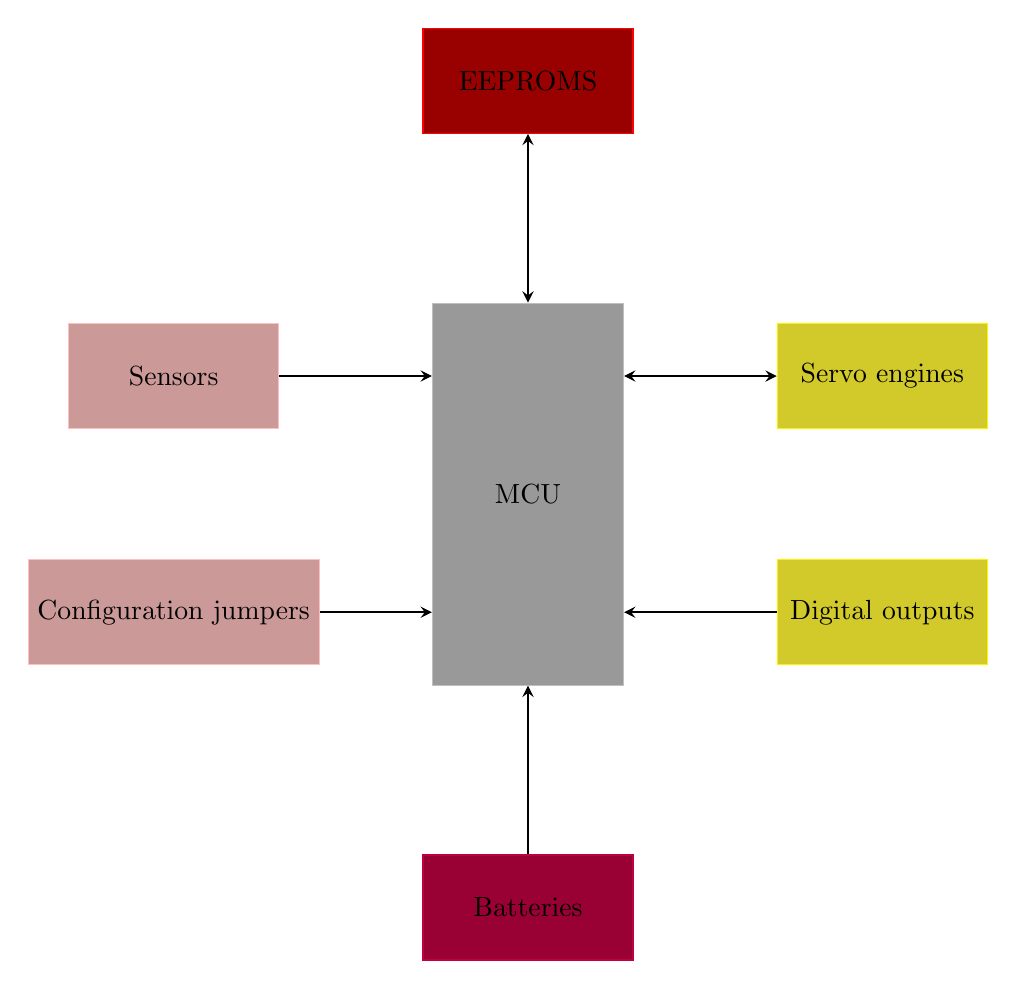
\begin{tikzpicture}[scale=0.75]
        % ---------------------------------------------------------------------------
        % Draw nodes
        % ---------------------------------------------------------------------------
        \node[  rectangle, 
                draw = lightgray, 
                text = black, 
                fill = lightgray!80!black, 
                minimum width = 0.2\textwidth, 
                minimum height = 0.4\textwidth]  (MCU) at (0,0) {MCU};

        \node[  rectangle, 
                draw = pink, 
                text = black, 
                fill = pink!80!black, 
                minimum width = 0.22\textwidth,
                minimum height = 0.11\textwidth]  (Sensors) at (-6,2) {Sensors};

        \node[  rectangle, 
                draw = pink, 
                text = black, 
                fill = pink!80!black, 
                minimum width = 0.22\textwidth, 
                minimum height = 0.11\textwidth]  (Jumpers) at (-6,-2) {Configuration jumpers};

        \node[  rectangle, 
                draw = yellow, 
                text = black, 
                fill = yellow!80!black, 
                minimum width = 0.22\textwidth, 
                minimum height = 0.11\textwidth]  (Outputs) at (6,-2) {Digital outputs};

        \node[  rectangle, 
                draw = yellow, 
                text = black, 
                fill = yellow!80!black, 
                minimum width = 0.22\textwidth, 
                minimum height = 0.11\textwidth]  (Engines) at (6,2) {Servo engines};

        \node[  rectangle, 
                draw = red, 
                text = black, 
                fill = red!60!black, 
                minimum width = 0.22\textwidth, 
                minimum height = 0.11\textwidth]  (EEPROMS) at (0,7) {EEPROMS};

        \node[  rectangle, 
                draw = purple, 
                text = black, 
                fill = purple!80!black, 
                minimum width = 0.22\textwidth, 
                minimum height = 0.11\textwidth]  (Batteries) at (0,-7) {Batteries};

        % ---------------------------------------------------------------------------
        % Draw arrows
        % ---------------------------------------------------------------------------
        \draw [-stealth, thick]             (Sensors.east)      -- (Sensors.east -| MCU.west);      % Sensors
        \draw [stealth-stealth, thick]      (Engines.west)      -- (Sensors.east -| MCU.east);      % Servo
        \draw [-stealth, thick]             (Jumpers.east)      -- (Jumpers.east -| MCU.west);      % Digital outputs
        \draw [-stealth, thick]             (Outputs.west)      -- (Outputs.west -| MCU.east);      % Config jumpers
        \draw [stealth-stealth, thick]      (EEPROMS.south)     -- (MCU.north);                     % EEPROMS
        \draw [-stealth, thick]             (Batteries.north)   -- (MCU.south);                     % Batteries
        
    \end{tikzpicture}
    
    \caption{Functional diagram of the electronic board}
    \label{fig:Functional}
\end{figure}